\documentclass[]{article}
\usepackage{lmodern}
\usepackage{amssymb,amsmath}
\usepackage{ifxetex,ifluatex}
\usepackage{fixltx2e} % provides \textsubscript
\ifnum 0\ifxetex 1\fi\ifluatex 1\fi=0 % if pdftex
  \usepackage[T1]{fontenc}
  \usepackage[utf8]{inputenc}
\else % if luatex or xelatex
  \ifxetex
    \usepackage{mathspec}
  \else
    \usepackage{fontspec}
  \fi
  \defaultfontfeatures{Ligatures=TeX,Scale=MatchLowercase}
\fi
% use upquote if available, for straight quotes in verbatim environments
\IfFileExists{upquote.sty}{\usepackage{upquote}}{}
% use microtype if available
\IfFileExists{microtype.sty}{%
\usepackage{microtype}
\UseMicrotypeSet[protrusion]{basicmath} % disable protrusion for tt fonts
}{}
\usepackage[margin=1in]{geometry}
\usepackage{hyperref}
\hypersetup{unicode=true,
            pdfborder={0 0 0},
            breaklinks=true}
\urlstyle{same}  % don't use monospace font for urls
\usepackage{color}
\usepackage{fancyvrb}
\newcommand{\VerbBar}{|}
\newcommand{\VERB}{\Verb[commandchars=\\\{\}]}
\DefineVerbatimEnvironment{Highlighting}{Verbatim}{commandchars=\\\{\}}
% Add ',fontsize=\small' for more characters per line
\usepackage{framed}
\definecolor{shadecolor}{RGB}{248,248,248}
\newenvironment{Shaded}{\begin{snugshade}}{\end{snugshade}}
\newcommand{\KeywordTok}[1]{\textcolor[rgb]{0.13,0.29,0.53}{\textbf{#1}}}
\newcommand{\DataTypeTok}[1]{\textcolor[rgb]{0.13,0.29,0.53}{#1}}
\newcommand{\DecValTok}[1]{\textcolor[rgb]{0.00,0.00,0.81}{#1}}
\newcommand{\BaseNTok}[1]{\textcolor[rgb]{0.00,0.00,0.81}{#1}}
\newcommand{\FloatTok}[1]{\textcolor[rgb]{0.00,0.00,0.81}{#1}}
\newcommand{\ConstantTok}[1]{\textcolor[rgb]{0.00,0.00,0.00}{#1}}
\newcommand{\CharTok}[1]{\textcolor[rgb]{0.31,0.60,0.02}{#1}}
\newcommand{\SpecialCharTok}[1]{\textcolor[rgb]{0.00,0.00,0.00}{#1}}
\newcommand{\StringTok}[1]{\textcolor[rgb]{0.31,0.60,0.02}{#1}}
\newcommand{\VerbatimStringTok}[1]{\textcolor[rgb]{0.31,0.60,0.02}{#1}}
\newcommand{\SpecialStringTok}[1]{\textcolor[rgb]{0.31,0.60,0.02}{#1}}
\newcommand{\ImportTok}[1]{#1}
\newcommand{\CommentTok}[1]{\textcolor[rgb]{0.56,0.35,0.01}{\textit{#1}}}
\newcommand{\DocumentationTok}[1]{\textcolor[rgb]{0.56,0.35,0.01}{\textbf{\textit{#1}}}}
\newcommand{\AnnotationTok}[1]{\textcolor[rgb]{0.56,0.35,0.01}{\textbf{\textit{#1}}}}
\newcommand{\CommentVarTok}[1]{\textcolor[rgb]{0.56,0.35,0.01}{\textbf{\textit{#1}}}}
\newcommand{\OtherTok}[1]{\textcolor[rgb]{0.56,0.35,0.01}{#1}}
\newcommand{\FunctionTok}[1]{\textcolor[rgb]{0.00,0.00,0.00}{#1}}
\newcommand{\VariableTok}[1]{\textcolor[rgb]{0.00,0.00,0.00}{#1}}
\newcommand{\ControlFlowTok}[1]{\textcolor[rgb]{0.13,0.29,0.53}{\textbf{#1}}}
\newcommand{\OperatorTok}[1]{\textcolor[rgb]{0.81,0.36,0.00}{\textbf{#1}}}
\newcommand{\BuiltInTok}[1]{#1}
\newcommand{\ExtensionTok}[1]{#1}
\newcommand{\PreprocessorTok}[1]{\textcolor[rgb]{0.56,0.35,0.01}{\textit{#1}}}
\newcommand{\AttributeTok}[1]{\textcolor[rgb]{0.77,0.63,0.00}{#1}}
\newcommand{\RegionMarkerTok}[1]{#1}
\newcommand{\InformationTok}[1]{\textcolor[rgb]{0.56,0.35,0.01}{\textbf{\textit{#1}}}}
\newcommand{\WarningTok}[1]{\textcolor[rgb]{0.56,0.35,0.01}{\textbf{\textit{#1}}}}
\newcommand{\AlertTok}[1]{\textcolor[rgb]{0.94,0.16,0.16}{#1}}
\newcommand{\ErrorTok}[1]{\textcolor[rgb]{0.64,0.00,0.00}{\textbf{#1}}}
\newcommand{\NormalTok}[1]{#1}
\usepackage{graphicx,grffile}
\makeatletter
\def\maxwidth{\ifdim\Gin@nat@width>\linewidth\linewidth\else\Gin@nat@width\fi}
\def\maxheight{\ifdim\Gin@nat@height>\textheight\textheight\else\Gin@nat@height\fi}
\makeatother
% Scale images if necessary, so that they will not overflow the page
% margins by default, and it is still possible to overwrite the defaults
% using explicit options in \includegraphics[width, height, ...]{}
\setkeys{Gin}{width=\maxwidth,height=\maxheight,keepaspectratio}
\IfFileExists{parskip.sty}{%
\usepackage{parskip}
}{% else
\setlength{\parindent}{0pt}
\setlength{\parskip}{6pt plus 2pt minus 1pt}
}
\setlength{\emergencystretch}{3em}  % prevent overfull lines
\providecommand{\tightlist}{%
  \setlength{\itemsep}{0pt}\setlength{\parskip}{0pt}}
\setcounter{secnumdepth}{0}
% Redefines (sub)paragraphs to behave more like sections
\ifx\paragraph\undefined\else
\let\oldparagraph\paragraph
\renewcommand{\paragraph}[1]{\oldparagraph{#1}\mbox{}}
\fi
\ifx\subparagraph\undefined\else
\let\oldsubparagraph\subparagraph
\renewcommand{\subparagraph}[1]{\oldsubparagraph{#1}\mbox{}}
\fi

%%% Use protect on footnotes to avoid problems with footnotes in titles
\let\rmarkdownfootnote\footnote%
\def\footnote{\protect\rmarkdownfootnote}

%%% Change title format to be more compact
\usepackage{titling}

% Create subtitle command for use in maketitle
\newcommand{\subtitle}[1]{
  \posttitle{
    \begin{center}\large#1\end{center}
    }
}

\setlength{\droptitle}{-2em}

  \title{STAT5101 Foundations of Data Science Assignment 3}
    \pretitle{\vspace{\droptitle}\centering\huge}
  \posttitle{\par}
    \author{Yiu Chung WONG 1155017920}
    \preauthor{\centering\large\emph}
  \postauthor{\par}
    \date{}
    \predate{}\postdate{}
  

\begin{document}
\maketitle

\subsubsection{1. A population has four members (called A, B, C, and D).
You would like to select a random sample of n = 2, which you decide to
do in the following way: Flip a coin; if it is heads, the sample will be
items A and B; if it is tails, the sample will be items C and D.
Although this is a random sample, it is not a simple random sample.
Explain
why.}\label{a-population-has-four-members-called-a-b-c-and-d.-you-would-like-to-select-a-random-sample-of-n-2-which-you-decide-to-do-in-the-following-way-flip-a-coin-if-it-is-heads-the-sample-will-be-items-a-and-b-if-it-is-tails-the-sample-will-be-items-c-and-d.-although-this-is-a-random-sample-it-is-not-a-simple-random-sample.-explain-why.}

A simple random sample is an individual being chosen randomly from the
population. In this setting, a group instead of a individual is being
chosen.

The combination of the two sample is predetermined. There is no chance
for A and D being selected together and same goes for B and C.

\subsubsection{2 The following data represent the number of days absent
per year in a population of six employees of a small
company:}\label{the-following-data-represent-the-number-of-days-absent-per-year-in-a-population-of-six-employees-of-a-small-company}

1 5 6 8 8 15

\subsubsection{Assuming that you sample with replacement, select all
possible samples of n = 2 and construct the sampling distribution of the
mean. Compute the mean of all sample means and also compute the
population mean. Are they equal? What is this property
called?}\label{assuming-that-you-sample-with-replacement-select-all-possible-samples-of-n-2-and-construct-the-sampling-distribution-of-the-mean.-compute-the-mean-of-all-sample-means-and-also-compute-the-population-mean.-are-they-equal-what-is-this-property-called}

\begin{Shaded}
\begin{Highlighting}[]
\NormalTok{population <-}\StringTok{ }\KeywordTok{c}\NormalTok{(}\DecValTok{1}\NormalTok{,}\DecValTok{5}\NormalTok{,}\DecValTok{6}\NormalTok{,}\DecValTok{8}\NormalTok{,}\DecValTok{8}\NormalTok{,}\DecValTok{15}\NormalTok{)}
\NormalTok{samples <-}\StringTok{ }\KeywordTok{t}\NormalTok{(}\KeywordTok{merge}\NormalTok{(population, population))}
\NormalTok{samples}
\end{Highlighting}
\end{Shaded}

\begin{verbatim}
##   [,1] [,2] [,3] [,4] [,5] [,6] [,7] [,8] [,9] [,10] [,11] [,12] [,13]
## x    1    5    6    8    8   15    1    5    6     8     8    15     1
## y    1    1    1    1    1    1    5    5    5     5     5     5     6
##   [,14] [,15] [,16] [,17] [,18] [,19] [,20] [,21] [,22] [,23] [,24] [,25]
## x     5     6     8     8    15     1     5     6     8     8    15     1
## y     6     6     6     6     6     8     8     8     8     8     8     8
##   [,26] [,27] [,28] [,29] [,30] [,31] [,32] [,33] [,34] [,35] [,36]
## x     5     6     8     8    15     1     5     6     8     8    15
## y     8     8     8     8     8    15    15    15    15    15    15
\end{verbatim}

\begin{Shaded}
\begin{Highlighting}[]
\NormalTok{means <-}\StringTok{ }\KeywordTok{data.frame}\NormalTok{(}\DataTypeTok{sample_means =} \KeywordTok{colMeans}\NormalTok{(samples))}
\KeywordTok{hist}\NormalTok{(means}\OperatorTok{$}\NormalTok{sample_means, }\DataTypeTok{main =} \StringTok{""}\NormalTok{, }\DataTypeTok{xlab =} \StringTok{"Sample Means"}\NormalTok{, }\DataTypeTok{prob =}\NormalTok{ T, }\DataTypeTok{col =} \StringTok{"darkred"}\NormalTok{)}
\KeywordTok{lines}\NormalTok{(}\KeywordTok{density}\NormalTok{(means}\OperatorTok{$}\NormalTok{sample_means), }\DataTypeTok{col =} \StringTok{"darkblue"}\NormalTok{, }\DataTypeTok{lwd =} \DecValTok{2}\NormalTok{)}
\KeywordTok{abline}\NormalTok{(}\DataTypeTok{v=}\KeywordTok{mean}\NormalTok{(means}\OperatorTok{$}\NormalTok{sample_means), }\DataTypeTok{col=}\StringTok{"black"}\NormalTok{)}
\end{Highlighting}
\end{Shaded}

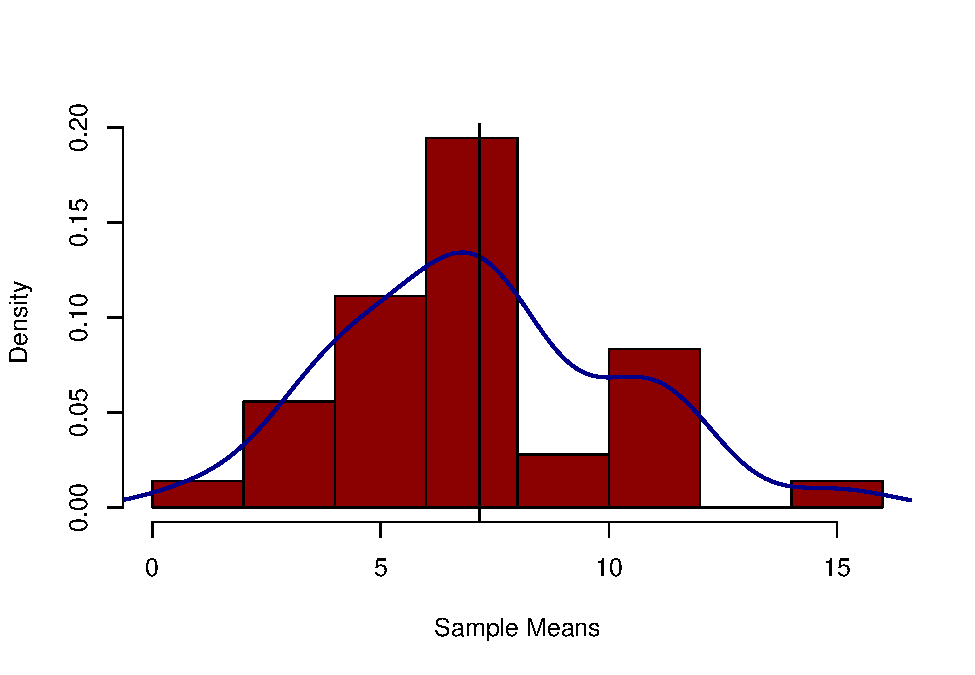
\includegraphics{Assignment_3_files/figure-latex/unnamed-chunk-2-1.pdf}

\begin{Shaded}
\begin{Highlighting}[]
\NormalTok{q2 <-}\StringTok{ }\KeywordTok{c}\NormalTok{(}\KeywordTok{mean}\NormalTok{(population), }\KeywordTok{mean}\NormalTok{(means}\OperatorTok{$}\NormalTok{sample_means))}
\KeywordTok{names}\NormalTok{(q2) <-}\StringTok{ }\KeywordTok{c}\NormalTok{(}\StringTok{"Population Mean"}\NormalTok{, }\StringTok{"Sample Mean"}\NormalTok{)}
\NormalTok{q2}
\end{Highlighting}
\end{Shaded}

\begin{verbatim}
## Population Mean     Sample Mean 
##        7.166667        7.166667
\end{verbatim}

\begin{itemize}
\tightlist
\item
  Sample means and the population mean are equal.
\item
  Central Limit Therom 
\end{itemize}

\subsubsection{3 The amount of time a bank teller spends with each
customer has a population mean μ = 3.10 minutes and standard deviation σ
= 0.40 minutes. Assume the population is symmetrically distributed, if a
random sample of 16 customers is
selected,}\label{the-amount-of-time-a-bank-teller-spends-with-each-customer-has-a-population-mean--3.10-minutes-and-standard-deviation--0.40-minutes.-assume-the-population-is-symmetrically-distributed-if-a-random-sample-of-16-customers-is-selected}

\paragraph{a) What is the probability that the average time spent per
customer will be at least 3
minutes?}\label{a-what-is-the-probability-that-the-average-time-spent-per-customer-will-be-at-least-3-minutes}

\begin{Shaded}
\begin{Highlighting}[]
\KeywordTok{pnorm}\NormalTok{(}\DataTypeTok{q =} \DecValTok{3}\NormalTok{, }\DataTypeTok{mean =} \FloatTok{3.10}\NormalTok{, }\DataTypeTok{sd =} \FloatTok{0.40} \OperatorTok{/}\StringTok{ }\KeywordTok{sqrt}\NormalTok{(}\DecValTok{16}\NormalTok{), }\DataTypeTok{lower.tail =} \OtherTok{FALSE}\NormalTok{)}
\end{Highlighting}
\end{Shaded}

\begin{verbatim}
## [1] 0.8413447
\end{verbatim}

\paragraph{b) There is an 85\% chance that the sample mean will be below
how many
minutes?}\label{b-there-is-an-85-chance-that-the-sample-mean-will-be-below-how-many-minutes}

\begin{Shaded}
\begin{Highlighting}[]
\KeywordTok{qnorm}\NormalTok{(}\DataTypeTok{p =}\NormalTok{ .}\DecValTok{85}\NormalTok{, }\DataTypeTok{mean =} \FloatTok{3.10}\NormalTok{, }\DataTypeTok{sd =} \FloatTok{0.40} \OperatorTok{/}\StringTok{ }\KeywordTok{sqrt}\NormalTok{(}\DecValTok{16}\NormalTok{))}
\end{Highlighting}
\end{Shaded}

\begin{verbatim}
## [1] 3.203643
\end{verbatim}

\paragraph{c) If a random sample of 64 customers is selected, there is
an 85\% chance that the sample mean will be below how many
minutes?}\label{c-if-a-random-sample-of-64-customers-is-selected-there-is-an-85-chance-that-the-sample-mean-will-be-below-how-many-minutes}

\begin{Shaded}
\begin{Highlighting}[]
\KeywordTok{qnorm}\NormalTok{(}\DataTypeTok{p =}\NormalTok{ .}\DecValTok{85}\NormalTok{, }\DataTypeTok{mean =} \FloatTok{3.10}\NormalTok{, }\DataTypeTok{sd =} \FloatTok{0.40} \OperatorTok{/}\StringTok{ }\KeywordTok{sqrt}\NormalTok{(}\DecValTok{64}\NormalTok{))}
\end{Highlighting}
\end{Shaded}

\begin{verbatim}
## [1] 3.151822
\end{verbatim}

\subsubsection{4 A study of women in corporate leadership was conducted
by Catalyst, a New York research organization. The study concluded that
slightly more than 15\% of corporate officers at Fortune 500 companies
are women. Suppose that you select a random sample of 200 corporate
officers, and the true proportion held by women is
0.15.}\label{a-study-of-women-in-corporate-leadership-was-conducted-by-catalyst-a-new-york-research-organization.-the-study-concluded-that-slightly-more-than-15-of-corporate-officers-at-fortune-500-companies-are-women.-suppose-that-you-select-a-random-sample-of-200-corporate-officers-and-the-true-proportion-held-by-women-is-0.15.}

\paragraph{a) What is the probability that in the sample, less than 15\%
of the corporate officers will be
women?}\label{a-what-is-the-probability-that-in-the-sample-less-than-15-of-the-corporate-officers-will-be-women}

\begin{Shaded}
\begin{Highlighting}[]
\NormalTok{n <-}\StringTok{ }\DecValTok{200}
\NormalTok{se <-}\StringTok{ }\KeywordTok{sqrt}\NormalTok{(}\FloatTok{0.15}\OperatorTok{*}\NormalTok{(}\DecValTok{1} \OperatorTok{-}\StringTok{ }\FloatTok{0.15}\NormalTok{)}\OperatorTok{/}\NormalTok{n)}
\NormalTok{mu <-}\StringTok{ }\FloatTok{0.15}
\KeywordTok{pnorm}\NormalTok{(}\DataTypeTok{q =} \FloatTok{0.15}\NormalTok{, }\DataTypeTok{mean =}\NormalTok{ mu, }\DataTypeTok{sd =}\NormalTok{ se)}
\end{Highlighting}
\end{Shaded}

\begin{verbatim}
## [1] 0.5
\end{verbatim}

\paragraph{b) What is the probability that in the sample, between 13\%
and 17\% of the corporate officers will be
women?}\label{b-what-is-the-probability-that-in-the-sample-between-13-and-17-of-the-corporate-officers-will-be-women}

\begin{Shaded}
\begin{Highlighting}[]
\NormalTok{n <-}\StringTok{ }\DecValTok{200}
\NormalTok{se <-}\StringTok{ }\KeywordTok{sqrt}\NormalTok{(}\FloatTok{0.15}\OperatorTok{*}\NormalTok{(}\DecValTok{1} \OperatorTok{-}\StringTok{ }\FloatTok{0.15}\NormalTok{)}\OperatorTok{/}\NormalTok{n)}
\NormalTok{mu <-}\StringTok{ }\FloatTok{0.15}
\KeywordTok{pnorm}\NormalTok{(}\DataTypeTok{q =} \FloatTok{0.17}\NormalTok{, }\DataTypeTok{mean =}\NormalTok{ mu, }\DataTypeTok{sd =}\NormalTok{ se) }\OperatorTok{-}\StringTok{ }\KeywordTok{pnorm}\NormalTok{(}\DataTypeTok{q =} \FloatTok{0.13}\NormalTok{, }\DataTypeTok{mean =}\NormalTok{ mu, }\DataTypeTok{sd =}\NormalTok{ se)}
\end{Highlighting}
\end{Shaded}

\begin{verbatim}
## [1] 0.5717081
\end{verbatim}

\subsubsection{5 Do ringing cell phones disturb business presentations?
In a poll of 326 business men and women, 303 answered this question
''yes'' and only 23 answered
''no''.}\label{do-ringing-cell-phones-disturb-business-presentations-in-a-poll-of-326-business-men-and-women-303-answered-this-question-yes-and-only-23-answered-no.}

\paragraph{a) Construct a 95\% confidence interval for the population
proportion of business men and women who have their presentations
disturbed by cell
phones.}\label{a-construct-a-95-confidence-interval-for-the-population-proportion-of-business-men-and-women-who-have-their-presentations-disturbed-by-cell-phones.}

\begin{Shaded}
\begin{Highlighting}[]
\NormalTok{p <-}\StringTok{ }\DecValTok{303}\OperatorTok{/}\DecValTok{326}
\NormalTok{z_value <-}\StringTok{ }\KeywordTok{qnorm}\NormalTok{(}\DataTypeTok{p =}\NormalTok{ .}\DecValTok{975}\NormalTok{)}
\NormalTok{se <-}\StringTok{ }\KeywordTok{sqrt}\NormalTok{(p }\OperatorTok{*}\StringTok{ }\NormalTok{(}\DecValTok{1} \OperatorTok{-}\StringTok{ }\NormalTok{p) }\OperatorTok{/}\StringTok{ }\DecValTok{326}\NormalTok{)}

\NormalTok{CI <-}\StringTok{ }\NormalTok{p }\OperatorTok{+}\StringTok{ }\KeywordTok{c}\NormalTok{(}\OperatorTok{-}\DecValTok{1}\NormalTok{, }\DecValTok{1}\NormalTok{) }\OperatorTok{*}\StringTok{ }\NormalTok{z_value }\OperatorTok{*}\StringTok{ }\NormalTok{se}
\NormalTok{CI}
\end{Highlighting}
\end{Shaded}

\begin{verbatim}
## [1] 0.9016503 0.9572454
\end{verbatim}

\paragraph{b) Interpret the interval constructed in
(a).}\label{b-interpret-the-interval-constructed-in-a.}

We are 95\% confident that the true percentage of people finding ringing
cell phones disturb business presentations in the population is between
90.2\% and 95.7\%.

Although the interval from 0.9016503 to 0.9572454 may or may not contain
the true proportion, 95\% of intervals formed from samples of size 326
in this manner will contain the true proportion.

\paragraph{c) If you were to conduct a follow-up study that would
provide 95\% confidence that the point estimate is correct to within
±0.04 of the population proportion, how large a sample size would be
required?}\label{c-if-you-were-to-conduct-a-follow-up-study-that-would-provide-95-confidence-that-the-point-estimate-is-correct-to-within-0.04-of-the-population-proportion-how-large-a-sample-size-would-be-required}

\begin{Shaded}
\begin{Highlighting}[]
\NormalTok{p <-}\StringTok{ }\DecValTok{303}\OperatorTok{/}\DecValTok{326}
\NormalTok{e <-}\StringTok{ }\FloatTok{0.04}
\NormalTok{z_value <-}\StringTok{ }\KeywordTok{qnorm}\NormalTok{(}\DataTypeTok{p =}\NormalTok{ .}\DecValTok{975}\NormalTok{)}

\NormalTok{n <-}\StringTok{ }\NormalTok{p }\OperatorTok{*}\StringTok{ }\NormalTok{(}\DecValTok{1} \OperatorTok{-}\StringTok{ }\NormalTok{p) }\OperatorTok{/}\StringTok{ }\NormalTok{(e}\OperatorTok{/}\NormalTok{z_value)}\OperatorTok{^}\DecValTok{2}

\KeywordTok{ceiling}\NormalTok{(n)}
\end{Highlighting}
\end{Shaded}

\begin{verbatim}
## [1] 158
\end{verbatim}

\subsubsection{6 The manager of a paint supply store wants to estimate
the actual amount of paint contained in 1- gallon cans purchased from a
nationally known manufacturer. It is known from the manufacturer's
specifications that the standard deviation of the amount of paint is
equal to 0.02 gallon. A random sample of 50 cans is selected, and the
sample mean amount of paint per 1-gallon can is 0.995
gallon.}\label{the-manager-of-a-paint-supply-store-wants-to-estimate-the-actual-amount-of-paint-contained-in-1--gallon-cans-purchased-from-a-nationally-known-manufacturer.-it-is-known-from-the-manufacturers-specifications-that-the-standard-deviation-of-the-amount-of-paint-is-equal-to-0.02-gallon.-a-random-sample-of-50-cans-is-selected-and-the-sample-mean-amount-of-paint-per-1-gallon-can-is-0.995-gallon.}

\paragraph{a) Set up a 99\% confidence inetrval estimate of the true
population mean amount of paint included in a 1-gallon
can.}\label{a-set-up-a-99-confidence-inetrval-estimate-of-the-true-population-mean-amount-of-paint-included-in-a-1-gallon-can.}

\begin{Shaded}
\begin{Highlighting}[]
\NormalTok{x_bar <-}\StringTok{ }\FloatTok{0.995}
\NormalTok{sigma <-}\StringTok{ }\FloatTok{0.02}
\NormalTok{z_value <-}\StringTok{ }\KeywordTok{qnorm}\NormalTok{(}\DataTypeTok{p =} \FloatTok{0.995}\NormalTok{)}
\NormalTok{n <-}\StringTok{ }\DecValTok{50}

\NormalTok{x_bar }\OperatorTok{+}\StringTok{ }\KeywordTok{c}\NormalTok{(}\OperatorTok{-}\DecValTok{1}\NormalTok{, }\DecValTok{1}\NormalTok{) }\OperatorTok{*}\StringTok{ }\NormalTok{z_value }\OperatorTok{*}\StringTok{ }\NormalTok{sigma}\OperatorTok{/}\KeywordTok{sqrt}\NormalTok{(n)}
\end{Highlighting}
\end{Shaded}

\begin{verbatim}
## [1] 0.9877145 1.0022855
\end{verbatim}

\paragraph{b) On the basis of your result in (a), do you think that the
manager has a right to complain to the manufacturer?
Why?}\label{b-on-the-basis-of-your-result-in-a-do-you-think-that-the-manager-has-a-right-to-complain-to-the-manufacturer-why}

No. The confidence interval contains the value 1; we are 95\% confident
that the true average volume of the paints is within this interval.
Since the value 1 is within this interval, we do not complain.

\paragraph{c) Does the population amount of paint per can have to be
normally distributed here?
Explain.}\label{c-does-the-population-amount-of-paint-per-can-have-to-be-normally-distributed-here-explain.}

No. According to Central Limit Therom, regardless the population
distribution, as long as we have a large sample size, the sample
distribution will approach normal.

\subsubsection{7 A consumer group wants to estimate the mean electric
bill for the month of July for single-family homes in a large city.
Based on studies conducted in other cities, the standard deviation is
assumed to be \$25. The group wants to estimate the mean bill for July
to within ± \$4 of the true average with 99\% confidence. What sample
size is
needed?}\label{a-consumer-group-wants-to-estimate-the-mean-electric-bill-for-the-month-of-july-for-single-family-homes-in-a-large-city.-based-on-studies-conducted-in-other-cities-the-standard-deviation-is-assumed-to-be-25.-the-group-wants-to-estimate-the-mean-bill-for-july-to-within-4-of-the-true-average-with-99-confidence.-what-sample-size-is-needed}

\begin{Shaded}
\begin{Highlighting}[]
\NormalTok{sigma <-}\StringTok{ }\DecValTok{25}
\NormalTok{e <-}\StringTok{ }\DecValTok{4}
\NormalTok{z_value <-}\StringTok{ }\KeywordTok{qnorm}\NormalTok{(}\DataTypeTok{p =} \FloatTok{0.995}\NormalTok{)}

\NormalTok{n <-}\StringTok{ }\NormalTok{(sigma }\OperatorTok{/}\StringTok{ }\NormalTok{(e}\OperatorTok{/}\NormalTok{z_value))}\OperatorTok{^}\DecValTok{2}
\KeywordTok{ceiling}\NormalTok{(n)}
\end{Highlighting}
\end{Shaded}

\begin{verbatim}
## [1] 260
\end{verbatim}


\end{document}
